\newpage
\section{Arhitektura sistema}
\subsection{Osnovni prikaz}
Sledi prikaz karakteristika arhitekture informacionog sistema za poručivanje hrane jednog restorana. Odluke su donošene u skladu sa prirodom i funkcionalnim zahtevima sistema, kao i potrebama korisnika i razvijaoca.Time su određene sledeće karakteristike arhitekture informacionog sistema:
\begin{enumerate}
    \item Tip aplikacije: Veb aplikacija
    \item Strategije isporučivanje: jedan serverski i više klijentskih računara
    \item Odgovarajuće tehnologije: Java, JavaFX, MYSQL, JS, CSS
    \item Prateće komponente:
    \begin{enumerate}
        \item \textbf{Logovanje na sistem:} Podsistem za autentikaciju korisnika. Sadrži GUI komponentu za učitavanje klijentskih podataka i komponentu za validaciju podataka.
        \item \textbf{Backup baze:} Predstavlja podsistem za pravljenje kopija baze. Uz to, vodi računa o konzistentnosti kopija, intervalu backup-ovanja i sl.
        \item \textbf{Pomoć:} Sadrži uputstvo za upotrebu, kontakt i podršku.
        
    \end{enumerate}
\end{enumerate}

\subsection{Tip arhitekture i slojevi}
Arhitektura sistema je osmišljena kao klijent-server tip arhitekture čiji su entiteti bazirani na tri (odnosno četiri) sloja.
\begin{enumerate}
    \item \textbf{Model} sadrži skup klasa koje opisuju sve entitete iz informacionog sistema. Model se sastoji od sledećih klasa sa opisanom funkcijom:
    \begin{itemize}
        \item \emph{Korisnik} je klasa koja sadrži sve lične informacije o korisniku aplikacije. Njegova polja su identična kolonama u tabeli Osoba (slika 11), takođe sadrži i alternativne adrese koje jedan korisnik može imati.
        \item \emph{Zaposleni} je klasa koja sadrži sve lične informacije o zaposlenom u restoranu. Polja klase Zaposleni identična su kolonama u tabeli Osoba (slika 11), takođe sadrži i informacije o njegovoj ulozi o sistemu, broj broj preostalih/iskorišćenih slobodnih dana, kao i podatak da li je taj zaposleni trenutno na odmoru.
        \item \emph{ZahtevZaOdsustvom} je klasa koja sadrži sva polja istoimenog entiteta. U ovoj klasi, nalaze se sve potrebne informacije za obradu zahteva zaposlenog za odlazak na plaćeno/neplaćeno odsustvo kao što su datum\_početka i datum\_završetka, kao i informacija o tome da li je određeni zahtev prihvaćen ili odbijen.
        \item \emph{Namirnica} je klasa oja sadrži podatke o svakoj namirnici koja se trenutno nalazi u magacinu. Ona direktno oslikava entitet Namirnice koji se nalazi u bazi.
         \item \emph{Jelo} je klasa koja oslikava prikaz jednog jela u jelovniku koji se prikazuje korisniku.
         \item \emph {Priprema} je klasa koja sadrži id-jeve klase Jelo i klase Namirnice i predstavlja njihovu agregaciju. Pruža nam informaciju o tome koje namirnice ulaze u sastav jednog jela.
         \item \emph{Porudžbina} je klasa koja sadrži sve informacije koje se prosleđuju nakon što korisnik uputi zahtev za poručivanjem određenog jela. Sadrži informacije o korisniku koji prosleđuje zahtev tj. id korisnika i propratne opisne informacije za datu porudžbinu.
         \item \emph{Spisak} je klasa koja sadrži id objekta klase Porudžbina, kao i listu id-jeva objekata klase Jelo. Informacije iz ove klase nam pomažu da vidimo koja sve jela ulaze u sastav jedne određene porudžbine, koja je njihova količina, kao i to da li je određeno jelo trenutno spremljeno ili se na njega čeka.
         \item \emph{Dostava} je klasa koja sadrži id porudžbine sa kojom je data dostava povezana, id zaposlenog koji će da izvrši dostavu. Beleže se i informacije o tome da li je određena dostava uspešno obavljena i koliko je vremena trebalo dostavljaču da izvrši dostavu. 
    \end{itemize}
    \item \textbf{View} odnosno pogled prikazuje podatke iz modela, u formatu pogodnom za interakciju, kao komponentu korisničkog interfejsa. Za svaki slučaj upotrebe kreiran je jedan view. U zavisnosti od toga da li je osoba koja poseduje nalog zaposleni u restoranu ili korisnik koji poručuje hranu, prikazuju im se različiti interfejsi nakon logovanja na sistem. Ono što im je zajedničko je kartica \emph{Nalog} koju imaju i korisnik i zaposleni. Ovde se nalaze sve njihove lične informacije koje su uneli tokom registracije, od kojih određene mogu da ažuriraju, uklone ili dodaju.
    \item \textbf{Kontroler} sadrži pripremu podataka za pogled, proračune, kao i njihovu pripremu pre slanja na obradu modelu. On je u ovom slučaju izdeljen na dve komponente - klijent, odnosno server kontroler. Klijentska strana obavlja komunikaciju između pogleda i modela u zavisnosti od korisnikovog unosa, dok se na serverskoj instanci obavlja autentikacija, autorizacija, i upravljanje podacima.
\end{enumerate}

\begin{figure}[!ht]
    \leavevmode
    \centering
    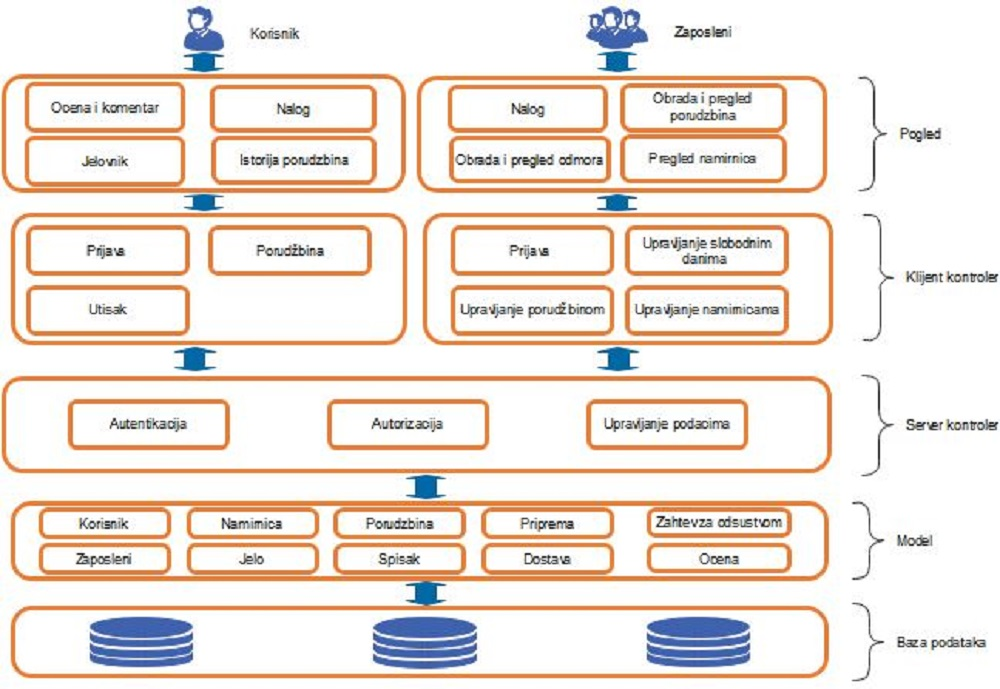
\includegraphics[width=1.2\textwidth]{slike/arhitektura.JPG}
    \caption{Arhitektura sistema}
    \label{fig:slika11}
\end{figure}
\leavevmode
